\chapter{Анализ предметной области}

В данной части рассматривается актуальность задачи, излагаются общие сведения об этапах, предшествующих распознаванию музыки по ритмическому паттерну, рассматриваются существующие методы распознавания музыкальных фрагментов на основе интерпретации ритма.

\section{Актуальность задачи}

В настоящее время технология распознавания музыки становится всё более востребованной \cite{bib14}. 

Ритм~---~один из наиболее фундаментальных элементов, позволяющих охарактеризовать музыкальный фрагмент \cite{bib2}. Обобщая, можно сказать, что совокупность ритмических последовательностей формирует структуру всего музыкального фрагмента, поэтому извлечение и анализ этих паттернов позволяет идентифицировать музыкальную композицию.

Вычислительная теория музыки предлагает широкий спектр интересных геометрических, комбинаторных и алгоритмических задач \cite{bib3}. Измерение сходства между ритмами является фундаментальной проблемой данной теории со многими приложениями, такими как поиск музыкальной композиции и решение проблем нарушений авторских прав \cite{bib2}.

\section{Постановка задачи и её приложения}

Под задачей распознавания музыки подразумевается перевод звукового сигнала в цифровое представление \cite{bib1}. Данное представление преобразовывается в массив данных, которые однозначно идентифицируют заданный фрагмент среди остальных. Обычно, наборы таких данных хранятся в базах данных. При необходимости распознать очередной фрагмент полученное представление сравнивается с другими представлениями музыкальных сигналов, которые уже хранятся в базе данных. Если выявляется совпадение, пользователь получает информацию об интересующем музыкальном фрагменте.

Технология распознавания музыки может решать следующие задачи:
\begin{itemize}
	\item задача поиска песни по музыкальному фрагменту;
	\item задача определения принадлежности песни к этнической культуре;
	\item задача нахождения сходства между музыкальными композициями;
	\item задача контроля соблюдения авторских прав.
\end{itemize}

\section{Этапы, предшествующие непосредственному распознаванию музыки}
\subsection{Интерпретация ритма}
Интерпретация ритма~---~вариант восприятия ритмического паттерна музыкального фрагмента человеком. Различные интерпретации будут далее рассмотрены на примере.
Одним из самых простых и популярных ритмов является $Clave$ $Son$, свойственный для танцевальной музыки, например, сальсы, и впервые появившийся на острове Куба \cite{bib3}. Для музыкантов данный ритм зачастую записывается с использованием стандартной нотной записи, варианты которой представлены на рисунке \ref{img:tab}.

\begin{figure}[h!]
    \centering
    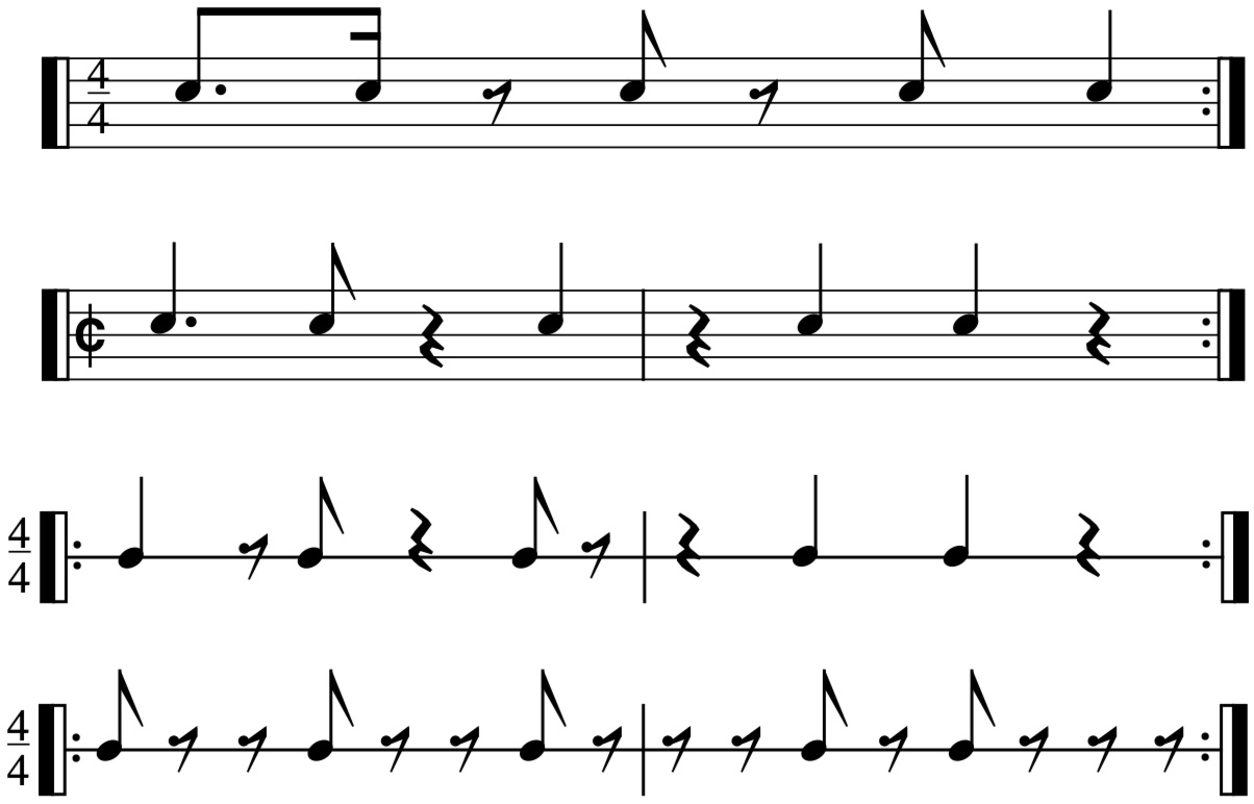
\includegraphics[scale=0.5]{img/tab.pdf}
    \caption{Стандартная нотная запись ритма $Clave$ $Son$ \cite{bib3}}
    \label{img:tab}
\end{figure}

Для многих ударников, не умеющих читать ноты, или обываталей, также не знакомых с музыкальной нотацией, данный ритм будет более понятен в  записи, указанной на рисунке \ref{img:box}.

\begin{figure}[h!]
    \centering
    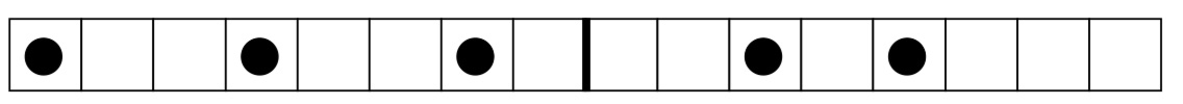
\includegraphics[scale=0.53]{img/box.pdf}
    \caption{$Box$ $Notation$ $Method$ записи ритма $Clave$ $Son$ \cite{bib3}}
    \label{img:box}
\end{figure}

Данный метод известен как $Box$ $Notation$ $Method$, разработанный Филипом Харландом из Калифорнийского университета в Лос-Анджелесе в 1962 году и также известный как $TUBS$ ($Time$ $Unit$ $Box$ $System$). Наличие выбранного символа в данной записи обозначает ноту, а отсутствие~---~паузу.

Аналогичны по смыслу и интерпретации на рисунке \ref{img:other}.

\begin{figure}[h!]
    \centering
    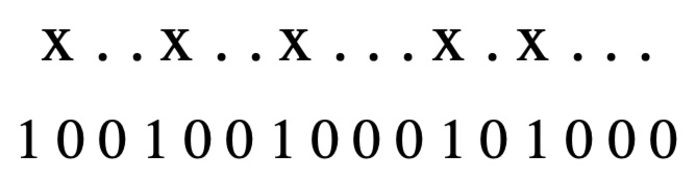
\includegraphics[scale=0.53]{img/other.pdf}
    \caption{Иные варианты интерпретации ритма без музыкальной нотации \cite{bib3}}
    \label{img:other}
\end{figure}

Немного отличным от предыдущих является вариант представления, при котором записываются в ряд числа, обозначающие длины интервалов между последовательными ударами. Данная интерпретация представлена на рисунке \ref{img:interv}.

\begin{figure}[h!]
    \centering
    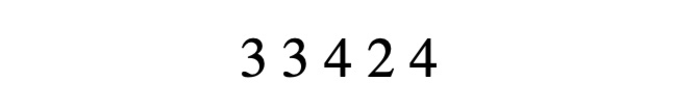
\includegraphics[scale=0.53]{img/interv.pdf}
    \caption{Интервальный вариант интерпретации ритма без музыкальной нотации \cite{bib3}}
    \label{img:interv}
\end{figure}

Существуют также геометрические варианты интерпретации ритма, например, в форме выпуклого многоугольника, что представлено на рисунке \ref{img:pol}.

\begin{figure}[h!]
    \centering
    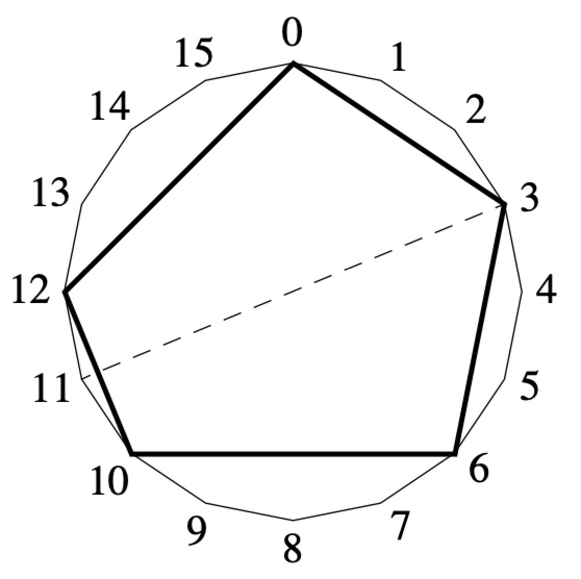
\includegraphics[scale=0.4]{img/pol.pdf}
    \caption{Геометрический вариант интерпретации ритма без музыкальной нотации \cite{bib3}}
    \label{img:pol}
\end{figure}

Данное представление более реалистично, потому что временные линии ритма цикличны, а все другие представления, рассмотренные выше, имеют начало и конец паттерна, расположенные физически на расстоянии друг от друга. При таком рассмотрении, ритм может быть представлен как вектор $X = (x_1, x_2, ..., x_n)$, где $x_i$ — число вершин, пропущенных $i$-м ребром многоугольника, начиная с вершины с номером 0.

\subsection{Транскрибирование}

Транскрибирование~---~это перевод содержания аудиофайла в символьный формат.

Могут быть выделены следующие виды транскрибирования:
\begin{enumerate}
	\item классифицирующие, среди которых использование скрытых марковских моделей и вероятностный анализ скрытых компонентов;
	\item нейросетевые, подразделяющиеся на одноуровневые и многоуровневые;
	\item комбинированные, например, с использованием адаптивных осцилляторов и нейросетей.
\end{enumerate}

Согласно источникам \cite{bib9} и \cite{bib10}, большинство перечисленных ниже методов транскрибирования применимы для ритмического транскрибирования.

\subsubsection{Автоматическое транскрибирование музыки с использованием моделей событий нот}

В источнике \cite{bib4} описано автоматическое транскрибирование музыки с использованием моделей событий нот. Данный метод предполагает наличие трёх вероятностных моделей~---~модели тишины и модели событий нот, представляющих собой скрытые марковские модели (HMM), и музыковедческой модели. Изначальные данные для транскрибирования обычно извлекаются из $MIDI$-файлов. Модель тишины моделирует временные области, в которых не звучат ноты, а события нот описываются с помощью скрытой модели с тремя состояниями, соответствующими типичным значениям признаков для нот. Музыковедческая модель, используя метод оценки музыкальной тональности, находит наиболее вероятные переходы между моделями нот и тишины. Схема взаимодействия моделей проиллюстрирована рисунком \ref{img:hmm}. 

\begin{figure}[h!]
    \centering
    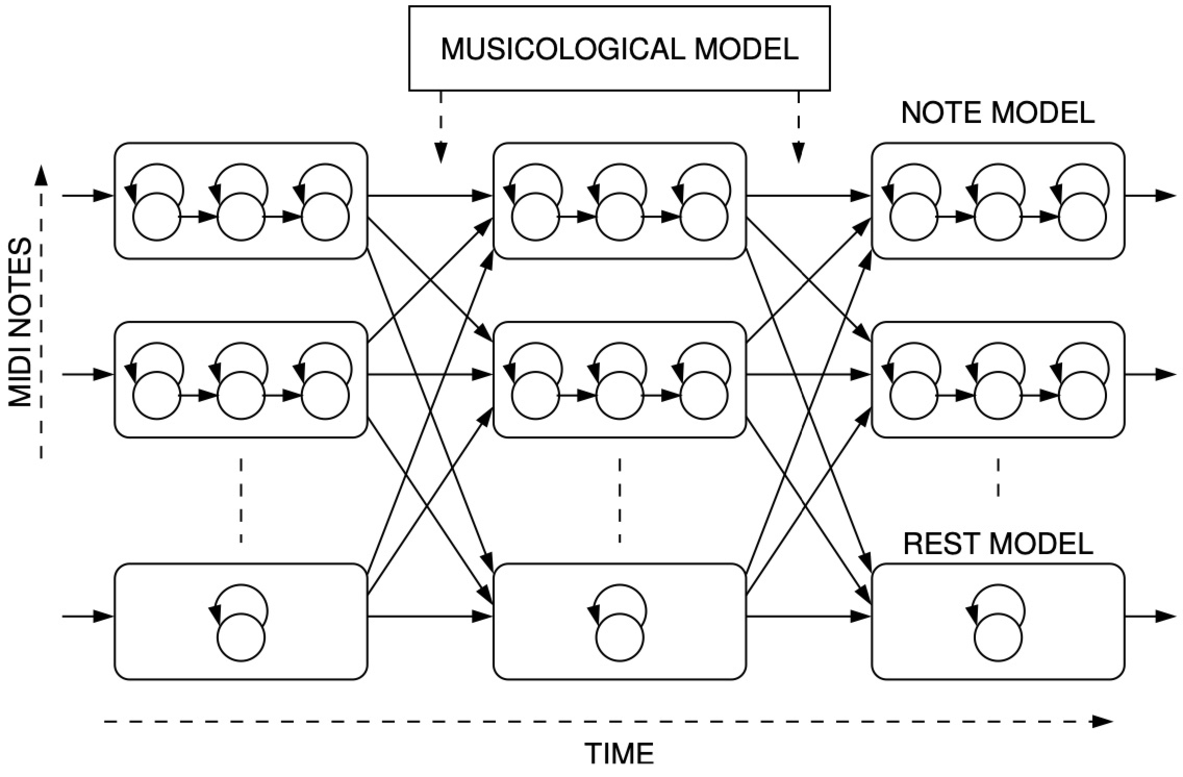
\includegraphics[scale=0.5]{img/hmm.pdf}
    \caption{Схема взаимодействия моделей при автоматическом транскрибировании музыки с использованием модели событий нот \cite{bib4}}
    \label{img:hmm}
\end{figure}

\subsubsection{Построение инвариантной к сдвигам модели скрытых переменных}

В источнике \cite{bib5} используется подход, представляющий собой построение инвариантной к сдвигам модели скрытых переменных. Основой подхода является теория вероятностного анализа скрытых компонентов \cite{bib6}, при котором входные спектрограммы аппроксимируются вероятностным распределением, зависящим от времени и частоты, а затем распределение раскладывается на отдельные спектральные компоненты. 

\subsubsection{Транскрибирование с помощью модели слухового восприятия}

В источнике \cite{bib7} использован "коннекционистский подход". Это означает, что музыкальный фрагмент рассматривается как набор элементов и сетевых связей между ними. Происходит переход от осциллограммы звукового сигнала к спектральному частотно-временному представлению с помощью модели слухового восприятия, полученной на основе бионических исследований слуха человека, и фильтрации звукового сигнала с частотным преобразованием. Элементами композиции, в рамках данного подхода, являются отдельные адаптивные осцилляторы, представляющие собой модели гармонических синусоидальных сигналов, адаптирующиеся под входящий сигнал с помощью нейросетевых методов. Сеть осцилляторов выделяет пики частот основного тона и обертонов. Каждый осциллятор отслеживает определённую ноту, подстраиваясь под входящий поток событий.

\subsubsection{Транскрибирование с помощью выявления во входящем звуковом сигнале онсетов}

В источнике \cite{bib8} используется выделение во фрагменте начал нот~---~онсетов. 
Метод основан на использовании сонограммы звуковой записи, которая в дальнейшем исследуется с помощью нейросетевых методов. Онсеты определяются в два этапа: сначала определяются те частотные полосы, в которых появились компоненты ноты, а потом определяется нота или ноты, способные породить такой набор частотных компонент. Поэтому для решения этой задачи строится двухуровневая нейронная сеть. Используемая нейронная сеть имеет два уровня. Первый уровень состоит из отдельных нейросетей, обучаемых на эталонных произведениях, для которых вручную описаны начало каждой ноты. Благодаря двухуровневой структуре верхний уровень позволяет корректировать результаты работы нейросетей нижнего уровня и получать более точные результаты.  

\section{Обзор методов распознавания музыкальных фрагментов на основе ритмической интерпретации}

После выбора метода интерпретации и транскрибирования музыкального фрагмента необходимо распознать музыкальный фрагмент на основе полученной ритмической картины. Для этого рассмотрим методы вычисления ритмического сходства музыкальных произведений.

В основе любого алгоритма распознавания музыкального фрагмента лежит задача определения сходства ритмической составляющей. Выбор метода решения этой задачи частично предопределен способом представления ритма. В соответствии с рассмотренными вариантами интерпретации ритма, рассмотрим методы измерения сходства двух ритмов, представленных последовательностями символов.

\subsection{Поиск редакционного расстояния}

Одним из наиболее распространённых методов распознавания музыкального фрагмента в ритмической записи последовательностью символов является поиск редакционного расстояния. Редакционное расстояние~---~это минимальное количество вставок, удалений и замен, необходимых для преобразования одной строки в другую. Для каждой операции над строкой вводится условная цена. Суммарная стоимость всех произведённых операций и будет являться редакционным расстоянием между данными строками.

Цены за редакционные операции можно обозначить  и определить следующим образом:
\begin{itemize}
	\item $\omega(\alpha,\beta)~=~1$~---~цена замены при $\alpha \neq \beta$;
	\item $\omega(\alpha,\alpha)~=~0$~---~цена эквивалентной замены;
	\item $\omega(\varnothing,\beta)~=~1$~---~цена вставки;
	\item $\omega(\alpha,\varnothing)~=~1$~---~цена удаления.
\end{itemize}

Для описания алгоритма вычисления редакционного расстояния, например, Левенштейна, применяется рекуррентное (т.е. использующее результаты предшествующих вычислений на следующем шаге) соотношение
\begin{equation}
\label{eqn:lev_formula}
	D(s_1[1..i], s_2[1..j]) = \begin{cases}
      	0,& \text{если}\ i = 0, j = 0, \\ 
        i,& \text{если}\ i > 0, j = 0, \\ 
        j,& \text{если}\ i = 0, j > 0, \\
     
      \min ( & D(s_1[1..i], s_2[1..j - 1]) + 1, \\
      & D(s_1[1..i - 1], s_2[1..j]) + 1, \\
      & D(s_1[1..i - 1], s_2[1..j - 1]) + m
      ),
      \end{cases}
\end{equation}
где
\begin{equation}
	m = \begin{cases}
      0, & \text{если}\ s_1[i] = s_2[j], \\
      1, & \text{иначе}. \\
      \end{cases}
\end{equation}

Таким образом, сходство с музыкальным фрагментом будет зафиксировано, если редакционное расстояние между их ритмической записью окажется минимальным.

\subsection{Поиск расстояния Хэмминга}

Для двоичных числовых последовательностей мерой сходства может являться расстояние Хэмминга, широко используемое в теории программирования. Расстояние Хэмминга~---~это количество позиций, где элементы не совпадают. Следовательно, это один из самых простых видов сопоставления шаблонов. При этом подходе каждый ритм представлен вектором $X = (x_1, x_2, ..., x_n)$, где $x_i$ представляют собой бинарные характеристики ритма. Если нота проигрывается в $i$-ю единицу времени, то $x_i$ = 1, иначе $x_i$ = 0. Таким образом, ритмы представляются точками в $n$-мерном бинарном векторном пространстве (гиперкубе). Расстояние Хэмминга между двумя точками $X = (x_1,x_2,...,x_n)$ и $Y = (y_1,y_2,...,y_n)$ в этом пространстве определяется выражением:
\begin{equation}
	d(X,Y) = \sum_{i = 1}^{n} \lvert x_i - y_i \rvert,
\end{equation}

Расстояние Хэмминга легко вычисляется за время $O(n)$. Данный метод выявляет наличие несоответствия, но не его величину.

\subsection{Поиск Евклидова интервального векторного расстояния}

Некоторые алгоритмы распознавания ритма и музыкальных паттернов используют интервалы между онсетами, то есть последовательными началами нот в ритме, в качестве основных признаков для измерения сходства. Этот подход и его варианты подходит для измерения подобия ритмов, больше, чем рассмотренные ранее, чем расстояние Хэмминга. 

Каждая ритмическая структура может быть представлена вектором чисел, совпадающих с длиной этих интервалов. Более конкретно, ритм может быть представлен вектором $X = (x_1, x_2, ..., x_n)$, где $x_i$~---~число вершин, пропущенных $i$-м ребром многоугольника, начиная с вершины, помеченной 0. 

По сути, это то же самое, что и последовательность временных интервалов между онсетами, поскольку временной интервал равен количеству пропущенных вершин, увеличенному на 1. Различие между двумя ритмами $X = (x_1, x_2, ..., x_n)$ и $Y = (y_1, y_2, ..., y_n)$ может быть вычислено с помощью Евклидова расстояния между двумя интервальными векторами $X$ и $Y$, в $n$-мерном векторном пространстве, как:
\begin{equation}
	d(X,Y) = \sqrt{\sum_{i = 1}^{n} (x_i - y_i)^2}.
\end{equation}

Векторы интервалов могут быть вычислены из заданных двоичных последовательностей за время $O(n)$, после чего Евклидово расстояние может быть вычислено за время $O(m)$, где $m$~---~количество онсетов, что приводит к итоговой оценке в $O(n)$.

\subsection{Поиск интервально-разностного векторного расстояния}

Музыкальный паттерн может быть представлен вектором разности ритмов \cite{bib11}. Если $T = (t_1, t_2,...,t_n)$~---~вектор интервалов времени между началами нот ритма (онсетами), то вектор разности ритма определяется как $X = (x_1, x_2,... , x_{n-1})$, где $x_i = \frac{t_i+1}{t_i}$. 

В контексте рассматриваемых здесь циклических ритмов $x_n = \frac{t_1}{t_n}$ размерность вектора разности ритмов будет равна $n$, а не $n-1$. Тогда пусть $X = (x_1,x_2,...,x_n)$ и $Y = (y_1,y_2,...,y_n)$ обозначают два интервально-разностных вектора. Различия между $X$ и $Y$ определяются следующим образом:
\begin{equation}
	d(X,Y) = \sum_{i = 1}^{n} \frac{max(x_i, y_i)}{min(x_i, y_i)} - n.
\end{equation}

Данная мера расстояния также вычисляется за время $O(n)$.

\subsection{Поиск обменного расстояния}

Задача сравнения двух двоичных строк одинаковой длины с одинаковым количеством единиц предполагает возможность проведения операции обмена. Обмен~---~это смена местами соседних единицы и нуля в двоичной строке. Расстояние перестановки между двумя ритмами~---~это минимальное количество обменов, необходимых для преобразования одного ритма в другой. Например, ритм, заданный последовательностью $[x . x . х х . x . x . x]$, где $x$ обозначает позицию онсета, можно преобразовать в ритмическую последолвательность $[x . x x . x x . x . x .]$ четырьмя обменами, а именно заменой третьей, пятой, шестой и седьмой доли на предшествующие им паузы. 
Разностное расстояние можно вычислить путем фактического выполнения перестановки, но это неэффективно \cite{bib12}. Если $X$ имеет единицы в первых $\frac{n}{2}$ позициях и нули в других местах, и если Y имеет единицы в последних $\frac{n}{2}$ позициях и нули в других, то потребуется по крайней мере квадратичное число обменов. С другой стороны, если вместо этого мы сравним вычисленные расстояния, получится гораздо более эффективный алгоритм. Сначала необходимо проанализировать двоичную последовательность и сохранить вектор позиций онсетов. Например, $X$ и $Y$ из примера выше дают векторы $U = (u_1,u_2,...,u_7) = (1,3,5,6,8,10,12)$ и $V = (v_1,v_2,... ,v_7) = (1,3,4,6,7,9,11)$ соответственно. Разница между $u_i$ и $v_i$ равна количеству обменов, которые необходимо выполнить, чтобы привести два вектора в соответствие. Следовательно, в общем случае расстояние перестановки между двумя векторами позиций онсетов $U$ и $V$ с $k$ онсетами определяется как:
\begin{equation}
	d(U,V) = \sum_{i = 1}^{n} \lvert u_i - v_i \rvert.
\end{equation}

Вычисление $U$ и $V$ из $X$ и $Y$ выполняется за время $O(n)$.

\subsection{Поиск хронотонического расстояния}
Далее рассматривается поиск хронотонического расстояния на примере. Пусть музыкальный фрагмент задан, как показано на рисунке \ref{img:chr1}.
\newpage
\begin{figure}[h!]
    \centering
    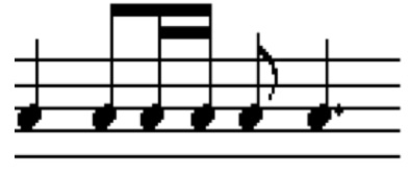
\includegraphics[scale=0.5]{img/chr1.pdf}
    \caption{Музыкальный фрагмент для поиска хронотонического расстояния \cite{bib13}}
    \label{img:chr1}
\end{figure}

Тогда хронотоническая цепочка может быть записана как $ch = [\frac{1}{4}, \frac{1}{8}, \frac{1}{16}, \frac{1}{16},\\ \frac{1}{8}, \frac{3}{8}]$. Видно, что кратчайшее время в цепочке~---~$\frac{1}{16}$ удара. Необходимо квантовать время на атомарные удары по $\frac{1}{16}$ удара. Теперь получается цепочка $ch = [4, 4, 4, 4, 2, 2, 1, 1, 2, 2, 6, 6, 6, 6, 6, 6] \cdot (\frac{1}{16})$. Данную цепочку можно изобразить на графике, по оси $x$ откладывая номер атомарного удара в последовательности, а по оси $y$~---~хронотоническое значение, как показано на рисунке \ref{img:chr2}.

\begin{figure}[h!]
    \centering
    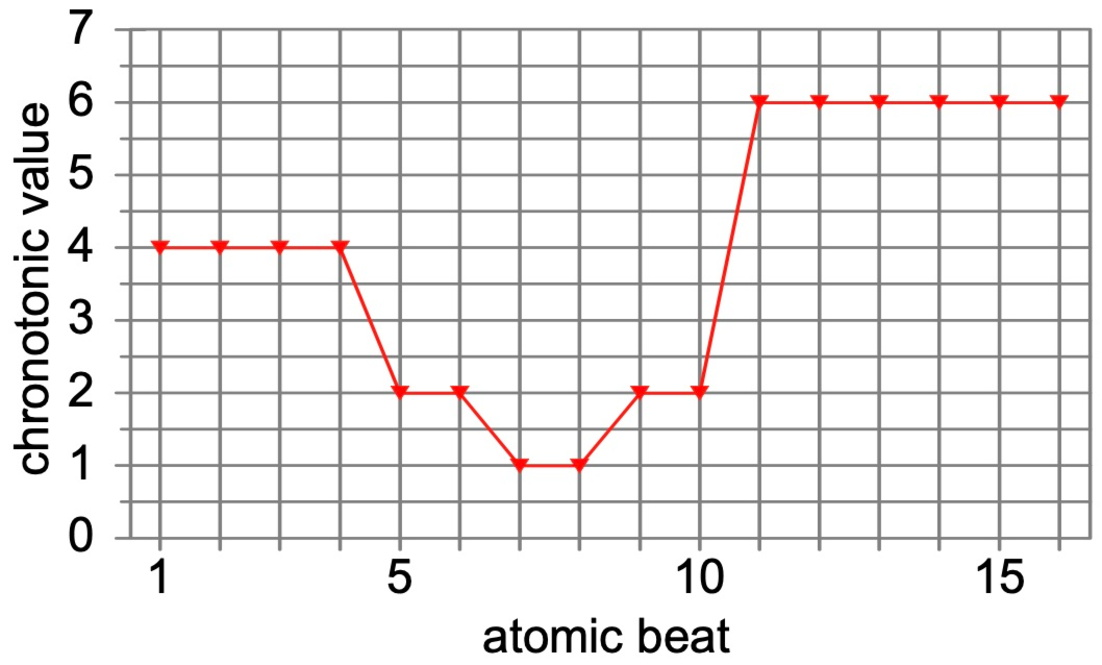
\includegraphics[scale=0.5]{img/chr2.pdf}
    \caption{Зависимость хронотонического значения от номера удара \cite{bib13}}
    \label{img:chr2}
\end{figure}

Если взять другую последовательноть, как на рисунке \ref{img:chr3}, то можно выполнить отображение первой последовательности на вторую, используя отражение графика одной из последовательностей относительно оси $x$.

\begin{figure}[h!]
    \centering
    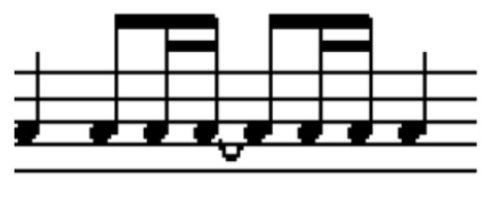
\includegraphics[scale=0.5]{img/chr3.pdf}
    \caption{Второй музыкальный фрагмент для поиска хронотонического расстояния \cite{bib13}}
    \label{img:chr3}
\end{figure}

Данную последовательность можно записать цепочкой $ch’ = [4, 4, 4, 4, 2, 2,\\ 1, 3, 3, 3, 1, 1, 4, 4, 4, 4] \cdot (\frac{1}{16})$. Проведённое отображение показано на рисунке \ref{img:chr4} тёмно-синим цветом. 

\begin{figure}[h!]
    \centering
    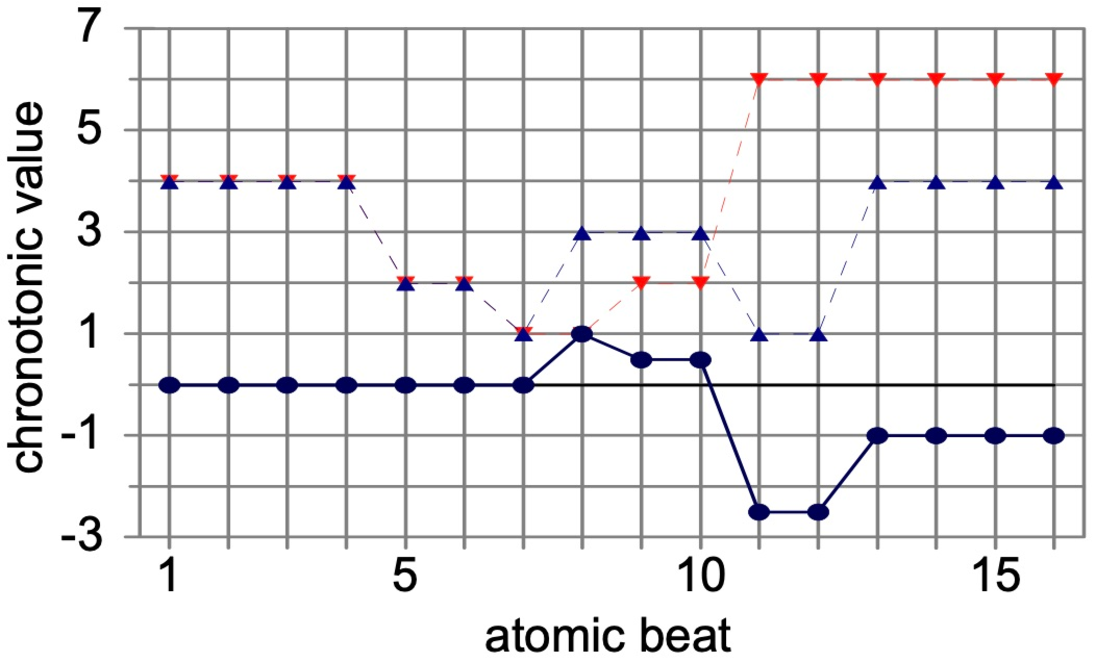
\includegraphics[scale=0.5]{img/chr4.pdf}
    \caption{Хронотоническое преобразование \cite{bib13}}
    \label{img:chr4}
\end{figure}

Такой механизм преобразования позволяет нам соотносить любые цепи одинаковой длины. Если две цепи имеют разную длину, необходимо увеличить более короткую цепь, чтобы она соответствовала более длинной цепи. 

Степень подобия между двумя цепочками определяется близостью цепочки отражения $R = [0, 0, 0, 0, 0, 0, 0, 1, 0.5, 0.5, -2.5, -2.5, 1, 1, 1, 1]$ и оси 0 $x$: чем они ближе, тем сильнее сходство.

Если взять две цепочки разной длины, то для уравнивания двух цепочек надо умножить хроноты (музыкальные длительности) одной цепочки на коэффициент $а$ (в случае, если, например, восьмые доли дополнить до четвертных, $а = 2$). Модель сходства не должна зависеть от соотношения длин цепочек, поэтому запишем формулу, соответствующую методу Шепарда:
\begin{equation}
	F_1 = e^{-k_1 \cdot ln^2(a)},
\end{equation}
где F1~---~показатель подобия, когда длина двух цепочек различна, то есть $\lvert ch \rvert = a \cdot \lvert ch’ \rvert$, а $k_1$~---~эмпирическая константа.

Далее нужно записать показатель подобия, связанный с цепочкой отражения $R = [r_1, r_2, ..., r_n]$, учитывая, что чем выше сходство, тем длиннее вектор:
\begin{equation}
	\lvert \lvert F_2 \rvert \rvert = \lvert \lvert \begin{pmatrix}
		\frac{e^{r_1^2 \cdot -\frac{k_2}{n}}}{\sqrt{n}} & \frac{e^{r_2^2 \cdot -\frac{k_2}{n}}}{\sqrt{n}} & ... & \frac{e^{r_n^2 \cdot -\frac{k_2}{n}}}{\sqrt{n}}
	\end{pmatrix}^T \rvert \rvert,
\end{equation}
что можно также записать как
\begin{equation}
	\lvert \lvert F_2 \rvert \rvert = \sqrt{
		\sum_{i = 1}^{n} (\frac{e^{r_i^2 \cdot -\frac{k_2}{n}}}{\sqrt{n}})^2},
\end{equation}
где $n$~---~длина цепочек в атомарных ударах (после выравнивания), $r_i$~---~$i$-я компонента цепочки отражения, $k_2$~---~эмпирическая постоянная.

Хронтоническое сходство будет выражаться в виде:
\begin{equation}
	S = F_1 \cdot \lvert \lvert F_2 \rvert \rvert.
\end{equation}

Описанная гипотеза была проверена в эксперименте \cite{bib13}.

\section{Вывод}

В данной части была рассмотрена актуальность задачи, изложены общие сведения об этапах, предшествующих распознаванию музыки по ритмическому паттерну, рассмотрены существующие методы распознавания музыкальных фрагментов на основе интерпретации ритма.

\newpage 

\chapter{Классификация методов распознавания музыкальных фрагментов на основе интерпретации ритма}

В данной части определяется критерий классификации методов распознавания музыкальных фрагментов на основе интерпретации ритма и проводится их классификация.

\section{Определение критерия классификации}

Согласно \cite{bib12}, в основе любого алгоритма распознавания музыкального фрагмента лежит задача определения сходства ритмической составляющей. Методы измерения сходства двух ритмов, представленных последовательностями символов, рассматривались, исходя из представленных в работе способов интерпретации ритма, поэтому будет проведена классификация именно по этому признаку.

\section{Классификация методов}

\subsection{Классификация методов по способу записи ритмического рисунка}
\par Исходя из полученного критерия, была получена схема классификации, которая выглядит следующим образом (\ref{img:class}).
\newpage

\begin{figure}[h!]
    \centering
    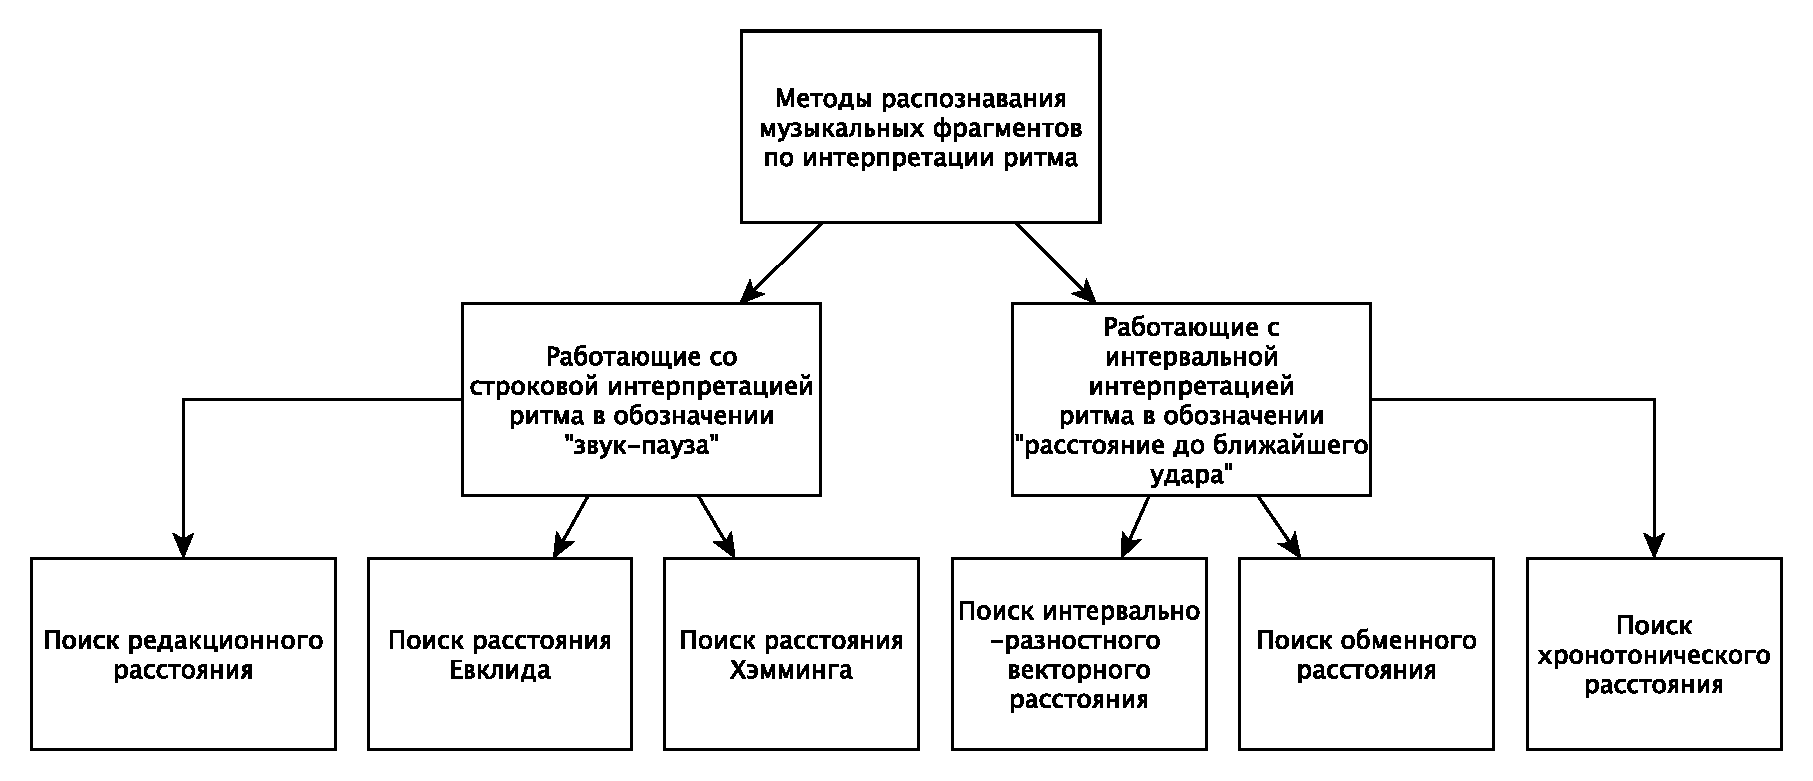
\includegraphics[scale=0.4]{img/class.pdf}
    \caption{Классификация методов распознавания музыкальных фрагментов на основе интерпретации ритма}
    \label{img:class}
\end{figure}

\subsection{Классификация методов по качественным характеристикам}
Кроме наиболее очевидного критерия классификации, можно также провести классификацию и сравнение перечисленных методов по  качественным критериям, указанным ниже. Автор источника \cite{bib12} проводит исследования данных методов распознавания музыкальных фрагментов на основе эксперимента по построению филогенетических деревьев. Данные деревья в контексте проводимого эксперимента отражают эволюционные взаимосвязи между бинарными и троичными ритмами двух семейств.

Сравнение проводится по следующим критериям:
\begin{enumerate}
	\item средний процент соответствия результатов работы методов действительной близости ритмов для двух семейств (avg fit \%);
	\item вычислительная сложность (complexity);
	\item соответствие соотношениям близости внутренних групп (clustering).
\end{enumerate}

В таблице \ref{tbl:class} представлена классификация и сравнение существующих методов распознавания музыкальных фрагментов на основе интерпретации ритма. Обозначения: РР~---~редакционное расстояние, РЕ~---~расстояние Евклида, РХ~---~расстояние Хэмминга, ИРВР~---~интервально-разностное векторное расстояние, ОР~---~обменное расстояние, ХР~---~хронотоническое расстояние.

\begin{table}[H]
	\begin{center}
		\centering
		\caption{Классификация и сравнение существующих методов распознавания музыкальных фрагментов на основе интерпретации ритма}
		\label{tbl:class}
		\begin{tabular}{|c|c|c|c|c|c|c|} 
			
			\hline
			\multicolumn{1}{|c|}{Критерий}
			&  \multicolumn{1}{c|}{РР}
			&  \multicolumn{1}{c|}{РЕ}
			&  \multicolumn{1}{c|}{РХ}
			&  \multicolumn{1}{c|}{ИРВР}
			&  \multicolumn{1}{c|}{ОР}
			&  \multicolumn{1}{c|}{ХР}\\
			\hline
			
			avg fit \% & -- & 85.15 & 75.1 & 43.3 & 100 & 100\\ \hline
			complexity & $O(n)$ & $O(n)$ & $O(n)$ & $O(n)$ & $O(n)$ & $O(n)$\\ \hline
			clustering & -- & Средне & Средне & Средне & Средне & Хорошо\\ \hline
			
		\end{tabular}
	\end{center}
\end{table}

В некоторых строках, соответствующих информации о методе поиска редакционного расстояния, нет информации о результатах исследования, так как автор источника \cite{bib12} не включал этот метод в рассмотрение.

\section{Вывод}

В данной части был определен критерий классификации существующих методов распознавания музыкальных фрагментов на основе интерпретации ритма и проведена их классификация и сравнение по качественным критериям.

\chapter*{Заключение}
\addcontentsline{toc}{chapter}{Заключение}

В ходе данной работы была выполнена поставленная цель: были рассмотрены существующие методы распознавания музыкальных фрагментов на основе интерпретации ритма и была проведена их классификация.

Задачи, решенные  для достижения поставленной цели:
\begin{enumerate}
    \item проведён анализ предметной области распознавания музыкальных фрагментов на основе интерпретации ритма;
    \item проведен обзор существующих методов распознавания музыкальных фрагментов на основе интерпретации ритма;
    \item сформулированы критерии их сравнения;
    \item классифицированы данные методы.
\end{enumerate}

